% BIL482 Dönem Projesi raporu (Türkçe). Overleaf'te pdfLaTeX ile derlenir.
% Şekiller: figures/tr/ (python -c "from hdtr import figures" ... ile sonuç dosyalarından üretilir).
\documentclass[conference,a4paper]{IEEEtran}
\usepackage[T1]{fontenc}
\usepackage[utf8]{inputenc}
\usepackage[turkish,shorthands=:!]{babel}
\usepackage{graphicx}
\usepackage{booktabs}
\usepackage{amsmath,amssymb}
\usepackage{multirow}
\usepackage{array}
\usepackage[normalem]{ulem}
\usepackage{xcolor}
\usepackage{tikz}
\usetikzlibrary{positioning,arrows.meta}
\usepackage[hidelinks]{hyperref}
\usepackage{cite}
\graphicspath{{figures/tr/}}
\raggedbottom

\begin{document}

\title{Türkçe RAG Cevaplarında Halüsinasyon Tespiti:\\ Tek Protokollü Karşılaştırma, Yeni Bir Dedektör\\ ve Özgün Türkçe Test Kümesi}

\author{\IEEEauthorblockN{İshak Türk}
\IEEEauthorblockA{Öğrenci No: 23120205003\\
BIL482 Dönem Projesi\\
Kod ve veri: \url{https://github.com/ishakturk/Turkish-RAG-Hallucination-Detector}}}

\maketitle

\begin{abstract}
Bilgi getirme destekli üretim (RAG) sistemleri, verilen bağlamda bulunmayan bilgileri de üretebilir. Bu çalışmada Türkçe RAG cevaplarında bu tür halüsinasyonları kelime ve karakter düzeyinde işaretleyen kodlayıcı (encoder) tabanlı dedektörleri inceliyoruz. Önce mevcut yedi Türkçe dedektörü ve iki klasik yöntemi tek ve tekrar üretilebilir bir protokolle değerlendirdik: tüm sistemler aynı karakterler üzerinden puanlandı, her sisteme kendi geliştirme kümesinde ayarlanmış eşik verildi ve test kümesi yalnızca bir kez açıldı. Önceden kaydedilmiş analiz planına göre nihai modelimiz (temizlenmiş RAGTruth-TR üzerinde ağırlıklı kayıpla ince ayarlanmış mmBERT-base), en iyi referans dedektöre göre örnek düzeyi F1'de $+0{,}070$ [0{,}049; 0{,}093] ve span düzeyi F1'de $+0{,}100$ [0{,}075; 0{,}125] puan daha iyidir; keşifsel karşılaştırmalarda mevcut yedi dedektörün tamamını geçmektedir. Kontrollü deneyler, kazancın büyük kısmının çok dilli temel modelden geldiğini, halüsinasyon ön eğitiminin ve veri artırmanın çeviri testte belirgin bir fayda sağlamadığını göstermektedir. Son olarak Qwen3-8B ve DeepSeek ile üretilmiş 184 cevaptan oluşan özgün bir Türkçe test kümesi oluşturduk. Bu kümede tüm denetimli dedektörlerin başarımı belirgin biçimde düşmektedir (nihai model: örnek F1 0{,}766 $\rightarrow$ 0{,}458); en iyi sonucu ise özgün Türkçe veriyle artırılmış model verir (0{,}592). Bulgular, makine çevirisiyle elde edilmiş testlerin Türkçe dedektörlerin gerçek başarımını olduğundan yüksek gösterdiğine işaret etmektedir.
\end{abstract}

\begin{IEEEkeywords}
halüsinasyon tespiti, RAG, Türkçe doğal dil işleme, span tespiti, kodlayıcı modeller, değerlendirme metodolojisi
\end{IEEEkeywords}

% ------------------------------------------------------------------------------------------------
\section{Giriş}

Büyük dil modelleri (BDM), bir soruyu cevaplarken dış kaynaklardan getirilen metinlere dayanacak şekilde kullanıldığında (RAG), cevabın bu metinlere \emph{sadık} olması beklenir. Ancak modeller zaman zaman bağlamda olmayan bir tarih, sayı veya iddia ekler. Bu çalışmada ``halüsinasyon'' ile, gerçek dünyada doğru olsa bile \emph{verilen bağlam tarafından desteklenmeyen} her ifadeyi kastediyoruz. Örneğin bağlam ``Lig 1927'de kuruldu'' derken cevabın ``Lig 1927'de kuruldu ve ilk şampiyonu Skonto FC oldu'' demesi, ikinci kısım bağlamda geçmediği için halüsinasyondur.

Pratikte bu sorun için iki yaklaşım vardır: cevabı başka bir BDM'ye kontrol ettirmek veya küçük bir kodlayıcı modeli cevaptaki her kelime için ``desteklenmiyor'' olasılığı verecek şekilde eğitmek. İkinci yaklaşım (ör. LettuceDetect~\cite{kovacs2025lettucedetect}) ucuz, hızlı ve yerel çalıştırılabilir olduğu için üretim sistemlerinde tercih edilir. Türkçe için bu alandaki tek kapsamlı çalışma Turk-LettuceDetect'tir~\cite{tas2025turk}: İngilizce RAGTruth~\cite{niu2024ragtruth} veri kümesi makine çevirisiyle Türkçeye aktarılmış (RAGTruth-TR) ve bu veri üzerinde birkaç kodlayıcı eğitilmiştir.

Mevcut Türkçe çalışmaları incelediğimizde üç eksik gördük. (i) Sonuçlar farklı düzeylerde ve tutarsız biçimde raporlanmıştır: makalede token düzeyinde makro F1 verilmiş, model kartlarında ise düzeyi belirtilmemiş farklı sayılar yer almaktadır; makaledeki tablolarda AUROC değerleri on iki satırın hepsinde geri çağırma (recall) değeriyle aynıdır, değerlendirme kodu da yayımlanmamıştır. (ii) Model seçimi ve eşik ayarı için ayrı bir doğrulama kümesi tanımlanmamıştır. (iii) Tüm değerlendirme çeviri metin üzerindedir; dedektörlerin \emph{doğal} Türkçe cevaplarda nasıl çalıştığı bilinmemektedir.

Bu çalışmanın katkıları şunlardır:
\begin{enumerate}
\item \textbf{Tek protokollü, tekrar üretilebilir karşılaştırma:} Mevcut yedi Türkçe/çok dilli dedektör ve iki klasik yöntem aynı veride, aynı kodla, karakter düzeyinde ortak metriklerle ve her sisteme geliştirme kümesinde ayarlanmış eşikle değerlendirildi. Karar kuralları test kümesi açılmadan önce yazılı bir analiz planına kaydedildi.
\item \textbf{Yeni bir dedektör:} mmBERT-base~\cite{marone2025mmbert} üzerine kurulan nihai modelimiz (R2), önceden belirlenmiş birincil karşılaştırmada en iyi referans dedektörü her iki birincil metrikte de anlamlı biçimde geçer; keşifsel karşılaştırmalarda mevcut tüm dedektörlerden iyidir.
\item \textbf{Kontrollü bulgular:} Türkçeye özgü (TabiBERT) ve çok dilli (mmBERT) temel modeller, halüsinasyon ön eğitimi, eğitim tarifi ve özgün Türkçe veri artırmanın etkisi aynı protokolle ölçüldü.
\item \textbf{Özgün Türkçe test kümesi:} Vikipedi ve Türk mevzuatı bağlamlarında, iki farklı BDM tarafından doğrudan Türkçe yazılmış 184 cevap; LLM ile etiketlenip 50 satırlık kör bir örneklemle insan tarafından doğrulandı. Bu küme, çeviri test ile gerçek kullanım arasındaki farkı ilk kez ölçmemizi sağladı.
\end{enumerate}

% ------------------------------------------------------------------------------------------------
\section{İlgili Çalışmalar}

\textbf{Veri kümeleri.} RAGTruth~\cite{niu2024ragtruth}, altı farklı BDM'nin soru-cevap (MS MARCO), veriden metin (Yelp) ve özetleme (haber) görevlerinde ürettiği yaklaşık 18 bin cevabı span düzeyinde etiketler ve bu alanın standart kaynağıdır. Çok dilli halüsinasyon kaynakları arasında HalluVerse25~\cite{abdaljalil2025halluverse25} ve HalluVerse-M3~\cite{abdaljalil2026halluversem3} Türkçe içerir, ancak bağlama dayalı span etiketleri sunmaz. MultiWikiQHalluA~\cite{thoresen2026multiwiki} çok dilli Vikipedi soru-cevap verisi üzerinde sentetik halüsinasyon üretir, fakat Türkçe alt kümesi yoktur.

\textbf{Kodlayıcı tabanlı dedektörler.} LettuceDetect~\cite{kovacs2025lettucedetect}, ModernBERT~\cite{warner2024modernbert} ile RAGTruth üzerinde token sınıflandırması yapar ve uzun bağlamı (8.192 token) tek seferde okuyabilir. Luna~\cite{belyi2025luna} benzer şekilde hafif bir değerlendirme modelidir; RAG-HAT~\cite{song2024raghat} ise halüsinasyona duyarlı ince ayar yapar. Dikkat özelliklerinden~\cite{ogasa2025multiview} ve zaman içindeki sinyallerden~\cite{itkin2026temporal} yararlanan yöntemler de önerilmiştir.

\textbf{Üretken dedektörler.} Son çalışmalar span tespitini pekiştirmeli öğrenmeyle eğitilmiş üretken modellerle yapar (RL4HS~\cite{su2025rl4hs}, SOPO~\cite{dong2026sopo}) veya kapsamı koda ve araç çıktılarına genişletir~\cite{kovacs2026beyond}. Bu yöntemler daha güçlü olabilir, ancak milyarlarca parametre gerektirir. SOPO'nun raporladığı span düzeyi F1 değerleri (LettuceDetect-Large için 58{,}9), aynı modelin örnek düzeyi F1'inden (79{,}22) çok farklıdır; bu durum, düzeylerin karıştırılmaması gerektiğini açıkça gösterir.

\textbf{Türkçe.} Turk-LettuceDetect~\cite{tas2025turk}, RAGTruth'u Gemma ile Türkçeye çevirir ve ModernBERT-tr, TurkEmbed4STS, EuroBERT gibi kodlayıcıları eğitir; aynı ekip daha sonra bge-m3 ve Ettin~\cite{weller2025ettin} tabanlı dedektörler yayımlamıştır. RAGTurk~\cite{kose2026ragturk} Türkçe RAG için genel uygulama önerileri sunar. Temel model olarak Türkçe için sıfırdan eğitilmiş TabiBERT~\cite{turker2025tabibert}, 1.800'den fazla dili kapsayan mmBERT~\cite{marone2025mmbert} ve Avrupa dillerine odaklanan EuroBERT~\cite{boizard2025eurobert} uzun bağlamı destekleyen güncel kodlayıcılardır.

% ------------------------------------------------------------------------------------------------
\section{Veri}

\subsection{RAGTruth-TR}
RAGTruth-TR, 2.965 kaynak örneğine (soru veya belge) verilmiş $6$'şar cevaptan oluşan toplam 17.790 Türkçe cevaptır: 15.090 eğitim ve 2.700 test (450 kaynak). Her satırda istem (talimat, bağlam ve soru), cevap ve cevap içindeki halüsinasyonlu karakter aralıkları bulunur. Veri kümesinde kaynak kimliği ve doğrulama bölmesi yoktur. Aynı kaynağa verilmiş altı cevap farklı kümelere düşerse model, test sırasında bağlamı ``ezberlemiş'' olur; bu nedenle kaynak kimliğini yeniden kurmamız gerekti.

\subsection{İngilizce aslıyla hizalama ve veri denetimi}
Türkçe satırların İngilizce RAGTruth cevap dosyasıyla aynı sırada olduğunu varsaydık ve bunu üç sinyalle (span sayısı, sayıların örtüşmesi, uzunluk oranı) doğruladık. Satırların \%99{,}99'u kontrolü geçti; böylece tüm cevaplara kaynak kimliği atanabildi. Hizalanmış veride çeviri kaynaklı hataları kurallarla taradık. Sınır dışı span, span sayısının İngilizceden farklı olması, tekrarlayan n-gram ve yarım kalmış cevap gibi ``kesin'' kurallar satırların \%1{,}06'sını (eğitimde 170, testte 19 satır) eledi. Ayrıca cevapların \%3{,}5'inde çevirinin İngilizcede olmayan bir sayı eklediğini bulduk (ör. ``5 pm'' $\rightarrow$ ``17:00''); bu, etiketlenmemiş bir desteksiz bilgi, yani etiket gürültüsüdür.

\subsection{Bölmeler}
Resmî test bölmesini kaynağa göre gruplayarak bir kez ikiye ayırdık: \textbf{geliştirme} kümesi (90 kaynak, 540 cevap; eşikler ve tüm model seçimleri için) ve \textbf{nihai test} (360 kaynak, 2.160 cevap; yalnızca bir kez puanlandı). Eğitim kaynaklarının \%5'i erken durdurma için doğrulama kümesi olarak ayrıldı (eğitim 14.334, doğrulama 756 cevap). Denetimden geçen ``temiz'' sürümler de saklandı (temiz nihai test: 2.146 cevap). Halüsinasyonlu cevap oranı görevden göreve değişir: testte veriden metin \%64, soru-cevap \%18, özetleme \%23.

\subsection{Özgün Türkçe veri artırma}
RAGTruth-TR'de özetleme görevi tüm sistemler için zayıf olduğundan, Türkçe Vikipedi tabanlı \texttt{multi-wiki-qa} (\texttt{tr}) verisinden~\cite{thoresen2026multiwiki} yeni eğitim örnekleri ürettik. DeepSeek (\texttt{deepseek-flash}, düşünme kapalı) her bağlam için önce bağlama sadık bir cevap veya özet yazdı; örneklerin yarısında da aynı metnin, her hatası \texttt{<HAL>}\ldots\texttt{</HAL>} etiketiyle işaretlenmiş hatalı bir sürümünü üretti. Hata türleri varlık değişimi, sayı/tarih değişimi, çelişki ve desteksiz ek bilgiydi. Etiketler karakter aralıklarına dönüştürüldü ve otomatik kurallarla denetlendi: dengesiz etiket, Türkçe olmayan metin, bağlamda olmayan sayı, değişmemiş metne konmuş etiket.

İlk istem sürümünde önemli bir kısayol bulduk: hatalı cevapların üçte biri, sona eklenmiş tek bir cümleden oluşuyordu. Bir model ``sondaki ek cümle halüsinasyondur'' kuralını öğrenebilirdi. İkinci sürümde hatalar cümle içine dağıtıldı ve son cümle oranı \%3{,}4'e indi (RAGTruth-TR: \%11). 30 örneklik kalite kapısında elle incelenen örneklerin 29'u kabul edildi. Tam çalıştırma 3.657 bağlamdan 5.484 kayıt üretti (\%33 halüsinasyonlu) ve toplam API maliyeti 0{,}80 dolar oldu. Bu veriyi yalnızca R4 modeli kullanır; artırma verisinin makaleleri, özgün test kümesinin makalelerinden ayrıdır.

\subsection{Özgün Türkçe test kümesi}
Çeviri test, dedektörlerin \emph{çeviri} Türkçesini ne kadar iyi okuduğunu ölçer. Doğal Türkçe cevaplardaki başarımı ölçmek için ayrı bir küme oluşturduk:
\begin{itemize}
\item \textbf{Bağlamlar:} veri artırmada kullanılmayan 133 Vikipedi makalesinden 139 ve \texttt{turkish-legal-rag} veri kümesindeki insan yazımı sorulardan (8 kanun) 45 bağlam, her biri en fazla 1.500 karakter.
\item \textbf{Sorular:} yarısı veri kümesinin orijinal sorusu; diğer yarısı, bağlamın yalnızca \emph{bir kısmını} cevapladığı biçimde yeniden yazılmış sorular (ör. bağlamda olan kuruluş yılına ek olarak, bağlamda olmayan ilk şampiyonu da sorma). Yeniden yazılan 203 sorunun tamamı elle incelendi; eksik bilginin aslında bağlamda bulunduğu 30 soru elendi.
\item \textbf{Cevaplar:} yarısı Colab'de çalıştırılan açık kaynaklı Qwen3-8B~\cite{yang2025qwen3}, yarısı DeepSeek API'si ile, dedektörlerin eğitildiği RAGTruth-TR soru şablonu kullanılarak üretildi. Yalnızca ``cevap verilemiyor'' diyen cevaplar elendi. DeepSeek soruların \%38'inde, Qwen \%9'unda doğrudan cevap vermeyi reddetti. Sonuçta 184 cevaplık bir küme elde edildi.
\end{itemize}

\textbf{Etiketleme.} Etiketleme kılavuzu (Türkçe ve İngilizce) cevaplar üretilmeden önce yazıldı; temel kural ``yalnızca bağlam geçerlidir'' idi. Kısmi cevaplar ve cevap vermeyi reddetme, söylenen her şey bağlamda olduğu sürece halüsinasyon sayılmadı. Referans etiketler iki bağımsız LLM (Claude) etiket kümesinden oluşturuldu; iki küme 184 satırın 178'inde uyuştu ($\kappa = 0{,}91$), uyuşmayan 6 satırı öğrenci karara bağladı. \textbf{İnsan doğrulaması} için tabakalı rastgele seçilmiş 50 satırı öğrenci, hiçbir yapay zekâ yardımı almadan ve etiketleme sırasında LLM etiketlerine bakmadan etiketledi (öğrenci daha önce tüm satırlar üzerindeki bir yapay zekâ geçişini görmüş olduğundan kontrol tam kör değildir; bkz. Sınırlılıklar). Etiketlenen 49 satırda uyum \%85{,}7, Cohen $\kappa = 0{,}38$ [$-0{,}07$; 0{,}73] çıktı (hukuk alanında 12/12 uyum). $\kappa$ değerinin düşük görünmesinin önemli bir nedeni, pozitif sınıfın seyrek olmasıdır (49 satırda yalnızca 6--7 halüsinasyon); yaygınlığa göre düzeltilmiş PABAK değeri 0{,}71'dir. Uyuşmayan 7 satır, iki tarafın notları görülerek kılavuza göre yeniden incelendi ve 6'sında LLM etiketi doğru bulundu. Bu satırlardaki farklar ya insan etiketleyicinin kaçırdığı ince desteksiz çıkarımlardı (ör. filmin yapım yılını ödül yılı olarak vermek) ya da kılavuza göre halüsinasyon sayılmayan eksik cevaplardı. Son referans kümede 184 cevabın 47'si (\%26) halüsinasyonludur. Halüsinasyonlu satırlardaki 52 span, desteklenmeyen kelimeleri tam olarak kapsayacak şekilde belirlendi.

Şekil~\ref{fig:rates}, halüsinasyon oranının üreten modele ve soru tipine çok güçlü biçimde bağlı olduğunu gösterir: Qwen3-8B cevaplarının \%44'ü, DeepSeek cevaplarının yalnızca \%4'ü halüsinasyonludur. Kısmen cevaplanabilir sorular, halüsinasyonun asıl tetikleyicisidir (\%45'e karşı \%9).

\begin{figure*}[t]
\centering
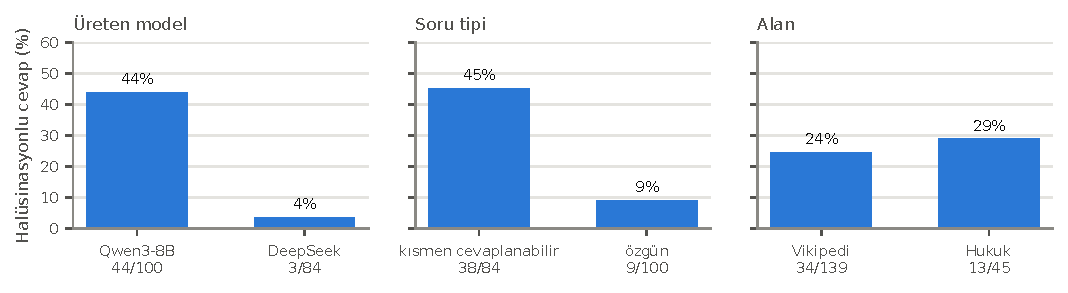
\includegraphics[width=\textwidth]{fig7_native_rates.pdf}
\caption{Özgün Türkçe test kümesinde halüsinasyonlu cevap oranı. Halüsinasyon büyük ölçüde Qwen3-8B'nin, bağlamın yalnızca bir kısmını cevapladığı sorulara verdiği cevaplarda ortaya çıkar.}
\label{fig:rates}
\end{figure*}

% ------------------------------------------------------------------------------------------------
\section{Yöntem}

\subsection{Görev tanımı}
Model girdisi \texttt{[CLS] istem [SEP] cevap [SEP]} biçimindedir. İstem token'larına etiket verilmez; cevaptaki her token, karakter aralığı herhangi bir altın span ile örtüşüyorsa 1 (halüsinasyon), aksi halde 0 olarak etiketlenir. Hizalama, hızlı tokenizer'ın karakter ofsetleriyle \emph{orijinal} metin üzerinde yapılır; Türkçedeki İ/ı sorunu nedeniyle metin hiçbir zaman bizim tarafımızdan küçük harfe çevrilmez. Farklı tokenizer'lara sahip modelleri adil karşılaştırmak için her model, cevabın her \emph{karakteri} için bir halüsinasyon olasılığı üretir (token olasılığı kapsadığı karakterlere dağıtılır). Tüm metrikler bu karakter olasılıklarından hesaplanır.

\begin{figure}[t]
\centering
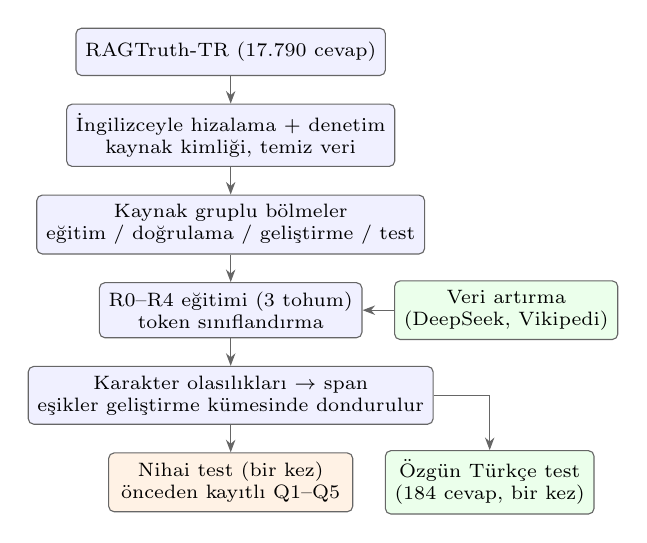
\begin{tikzpicture}[node distance=3.5mm, every node/.style={font=\scriptsize}, box/.style={draw=black!60, rounded corners=2pt, align=center, minimum width=3.1cm, minimum height=6mm, fill=blue!6}, arr/.style={-{Stealth[length=1.6mm]}, black!60}]
\node[box] (a) {RAGTruth-TR (17.790 cevap)};
\node[box, below=of a] (b) {İngilizceyle hizalama + denetim\\ kaynak kimliği, temiz veri};
\node[box, below=of b] (c) {Kaynak gruplu bölmeler\\ eğitim / doğrulama / geliştirme / test};
\node[box, below=of c] (d) {R0--R4 eğitimi (3 tohum)\\ token sınıflandırma};
\node[box, below=of d] (e) {Karakter olasılıkları $\rightarrow$ span\\ eşikler geliştirme kümesinde dondurulur};
\node[box, below=of e, fill=orange!10] (f) {Nihai test (bir kez)\\ önceden kayıtlı Q1--Q5};
\node[box, right=4mm of d, minimum width=2.4cm, fill=green!8] (g) {Veri artırma\\ (DeepSeek, Vikipedi)};
\node[box, right=4mm of f, minimum width=2.4cm, fill=green!8] (h) {Özgün Türkçe test\\ (184 cevap, bir kez)};
\draw[arr] (a)--(b); \draw[arr] (b)--(c); \draw[arr] (c)--(d); \draw[arr] (d)--(e); \draw[arr] (e)--(f);
\draw[arr] (g)--(d); \draw[arr] (e.east) -| (h.north);
\end{tikzpicture}
\caption{Çalışmanın akışı. Eşikler ve karar kuralları test açılmadan önce donduruldu.}
\label{fig:pipeline}
\end{figure}

\subsection{Modeller}
Tablo~\ref{tab:runs} eğittiğimiz beş model grubunu özetler. Her grup bir soruyu yanıtlamak için tasarlandı: R0 ile R1 yalnızca eğitim tarifinde, R1 ile R2 yalnızca temel modelde, R2 ile R3 yalnızca başlangıç ağırlıklarında, R2 ile R4 ise yalnızca veri artırmada farklıdır.

\begin{table}[t]
\centering
\caption{Eğitilen model grupları}
\label{tab:runs}
\footnotesize
\begin{tabular}{@{}lp{2.0cm}p{3.6cm}@{}}
\toprule
Grup & Temel model & Fark \\
\midrule
R0 & TabiBERT (149M) & Newmind tarzı tarif: 6 sabit devir, sade kayıp, temizlenmemiş veri, 1 tohum \\
R1 & TabiBERT (149M) & Bizim tarifimiz (aşağıda), temiz veri \\
R2 & mmBERT-base (307M) & R1 ile aynı tarif, çok dilli temel \\
R3 & KR Labs v2 mmBERT & R2 ile aynı mimari; İngilizce ve altı dilde halüsinasyon tespiti için önceden eğitilmiş \\
R4 & mmBERT-base & R2 + DeepSeek veri artırma (eğitimin \%25'i) \\
\bottomrule
\end{tabular}
\end{table}

\subsection{Eğitim tarifi}
AdamW (öğrenme oranı $3\cdot10^{-5}$, \%6 ısınma, doğrusal azalma, ağırlık azaltma 0{,}01), etkin yığın boyutu 16 ve en fazla 4 devir kullandık. Kayıp fonksiyonu sınıf ağırlıklı çapraz entropidir (pozitif sınıf ağırlığı $\sqrt{\text{negatif}/\text{pozitif}}$). Pilot çalışmada odak kaybı (focal loss) daha kötü sonuç verdiği için kullanılmadı. Doğrulama kelime F1'i her yarım devirde ölçüldü; 2 ölçüm boyunca iyileşme olmazsa eğitim durduruldu ve en iyi kontrol noktası seçildi. R1--R4 üç tohumla (42, 1234, 2026) eğitildi. Eğitimde istem ve cevap en fazla 4.096 token'a kadar okunur; sığmayan durumlarda cevap korunur, yalnızca istem kısaltılır (her eğitimde en fazla bir örnek). Çıkarımda sınır 8.192 token'dır; geliştirme ve özgün kümede hiçbir örnek kısaltılmadı. Bir mmBERT-base eğitimi tek bir NVIDIA L4 GPU'da yaklaşık bir saat sürdü. Tüm ayarlar Tablo~\ref{tab:hparams}'te ve depodaki \texttt{configs/} dosyalarındadır.

\begin{table}[t]
\centering
\caption{Eğitim ayarları (yığın: etkin yığın boyutu, yani yığın $\times$ gradyan biriktirme)}
\label{tab:hparams}
\scriptsize
\setlength{\tabcolsep}{3.5pt}
\begin{tabular}{@{}lcccccc@{}}
\toprule
Grup & Öğr.\ oranı & Devir & Yığın & Kayıp & Isınma & Erken durdurma \\
\midrule
R0 & $1\cdot10^{-5}$ & 6 (sabit) & 4 & sade CE & yok & yok \\
R1 & $3\cdot10^{-5}$ & $\leq$4 & 16 & ağırlıklı CE & \%6 & 2 ölçüm \\
R2 & $3\cdot10^{-5}$ & $\leq$4 & 16 & ağırlıklı CE & \%6 & 2 ölçüm \\
R3 & $3\cdot10^{-5}$ & $\leq$4 & 16 & ağırlıklı CE & \%6 & 2 ölçüm \\
R4 & \multicolumn{6}{c}{R2 ile aynı; eğitim örneklerinin \%25'ine kadar artırma verisi} \\
\bottomrule
\end{tabular}
\end{table}

\subsection{Son işleme ve eşikler}
Bir kelimenin en yüksek karakter olasılığı eşiği ($\tau$) geçerse kelime işaretlenir; Türkçe ekler kesme işaretiyle birlikte köke bağlı kalır (``Ocak'a''). Aralarında en fazla bir kısa kelime veya noktalama bulunan işaretli kelimeler tek span'de birleştirilir; 2 karakterden kısa span'ler atılır. Her sistem için, referans dedektörler dahil, iki eşik geliştirme kümesinde 0{,}05 adımlarla seçildi: örnek F1'i en yükselten $\tau_{\text{örnek}}$ ve span F1'i en yükselten $\tau_{\text{span}}$. Eşikler, nihai test açılmadan önce bir git commit'iyle donduruldu.

\subsection{Referans sistemler}
Newmind'ın altı Türkçe dedektörü (ModernBERT-tr, TurkEmbed4STS, EuroBERT-tr, bge-m3, Ettin-150M, Ettin-32M), Türkçe görmemiş KR Labs v2 mmBERT (sıfır atış) ve iki klasik yöntem: cevap cümlelerini bağlam cümleleriyle TF-IDF benzerliğiyle karşılaştıran sözcük örtüşmesi ve kelime düzeyinde (kelime bağlamda var mı, sayı mı, kök eşleşmesi vb.) lojistik regresyon. Geliştirme kümesinde en yüksek seçim puanını alan mevcut dedektör (TurkEmbed4STS) ``en iyi referans'' olarak önceden belirlendi.

\subsection{Metrikler ve istatistiksel çıkarım}
Birincil metrikler, halüsinasyon sınıfı için \textbf{örnek düzeyi F1} (cevapta en az bir tahmin edilen span var mı?) ve \textbf{span düzeyi F1}'dir (karakter örtüşmesine göre kesinlik ve geri çağırma, LettuceDetect'teki gibi). İkincil metrikler kelime F1'i ve AUROC'tur. Belirsizlik, \emph{kaynaklar} yeniden örneklenerek (aynı kaynağın altı cevabı birlikte) 2.000 tekrarlı bootstrap ile tahmin edildi; birden fazla tohumu olan modellerde her tekrarda tohum ortalaması alındı. Birincil soru (Q1) için karar kuralı önceden yazıldı: farkın \%95 güven aralığı (GA) tamamen sıfırın üstündeyse model ``daha iyidir''. Ayrıca her tohum için 10.000 permütasyonlu eşleştirilmiş permütasyon testi yapıldı. Q2--Q5 ikincil sorulardır ve çoklu karşılaştırma düzeltmesi yapılmadan etki büyüklüğü olarak raporlanır.

% ------------------------------------------------------------------------------------------------
\section{Sonuçlar}

\subsection{Birincil sonuç: nihai model en iyi referansı geçiyor}
Kurala göre nihai model R2 seçildi (geliştirme kümesinde R4'ün puanı R2'den düşük kaldı). Nihai testte R2, en iyi referans TurkEmbed4STS'e göre örnek F1'de $+0{,}070$ [0{,}049; 0{,}093] ve span F1'de $+0{,}100$ [0{,}075; 0{,}125] daha iyidir. Permütasyon testi her tohum ve her iki metrik için $p<0{,}001$ verir. Q1 iddiası bu nedenle sağlamdır. Tüm sistemlerin sonuçları Tablo~\ref{tab:main}'de ve Şekil~\ref{fig:main}'de verilmiştir; denetimden geçen temiz testte de tüm sonuçlar aynıdır.

\begin{table*}[t]
\centering
\caption{Nihai test (2.160 cevap) sonuçları, dondurulmuş geliştirme eşikleriyle. Bizim modellerimizde 3 tohumun ortalaması $\pm$ standart sapma; köşeli parantezler \%95 bootstrap güven aralığıdır.}
\label{tab:main}
\footnotesize
\begin{tabular}{@{}llccccc@{}}
\toprule
Sistem & Tür & Örnek F1 & Örnek F1 \%95 GA & Span F1 & Span F1 \%95 GA & Örnek AUROC \\
\midrule
\textbf{R2 mmBERT-base (nihai)} & bizim & \textbf{0,766 $\pm$ 0,003} & [0,738; 0,792] & \textbf{0,538 $\pm$ 0,003} & [0,493; 0,578] & \textbf{0,897} \\
R4 mmBERT + veri artırma & bizim & 0,748 $\pm$ 0,005 & [0,720; 0,774] & 0,534 $\pm$ 0,010 & [0,484; 0,573] & 0,888 \\
R3 KR Labs başlangıçlı & bizim & 0,761 $\pm$ 0,019 & [0,733; 0,785] & 0,525 $\pm$ 0,013 & [0,477; 0,570] & 0,896 \\
R1 TabiBERT & bizim & 0,716 $\pm$ 0,025 & [0,686; 0,743] & 0,487 $\pm$ 0,022 & [0,437; 0,531] & 0,870 \\
R0 TabiBERT, Newmind tarifi & bizim & 0,738 & [0,705; 0,767] & 0,471 & [0,417; 0,516] & 0,864 \\
\midrule
ModernBERT-tr & mevcut & 0,738 & [0,709; 0,765] & 0,470 & [0,423; 0,510] & 0,868 \\
bge-m3 & mevcut & 0,729 & [0,695; 0,760] & 0,469 & [0,421; 0,508] & 0,868 \\
EuroBERT-tr & mevcut & 0,714 & [0,679; 0,745] & 0,456 & [0,402; 0,501] & 0,859 \\
TurkEmbed4STS (en iyi referans) & mevcut & 0,696 & [0,661; 0,728] & 0,438 & [0,395; 0,474] & 0,851 \\
Ettin-150M & mevcut & 0,675 & [0,642; 0,705] & 0,413 & [0,367; 0,457] & 0,834 \\
Ettin-32M & mevcut & 0,644 & [0,608; 0,676] & 0,390 & [0,329; 0,446] & 0,787 \\
KR Labs v2 (sıfır atış) & mevcut & 0,551 & [0,519; 0,582] & 0,254 & [0,219; 0,298] & 0,699 \\
\midrule
Kelime lojistik regresyon & klasik & 0,615 & [0,584; 0,644] & 0,156 & [0,138; 0,176] & 0,758 \\
Sözcük örtüşmesi & klasik & 0,607 & [0,575; 0,637] & 0,141 & [0,127; 0,155] & 0,750 \\
\bottomrule
\end{tabular}
\end{table*}

\begin{figure*}[t]
\centering
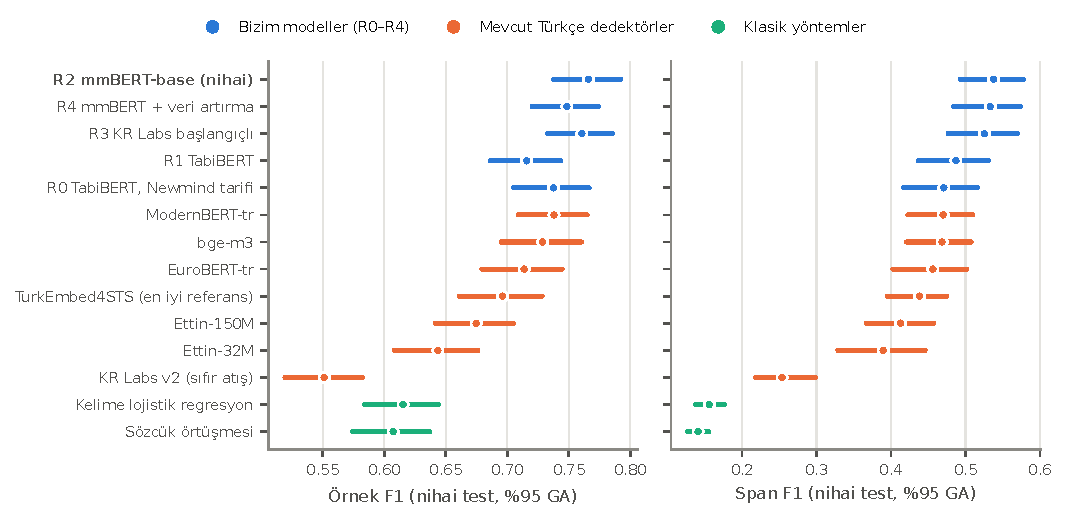
\includegraphics[width=\textwidth]{fig1_main_results.pdf}
\caption{Nihai testte tüm sistemlerin örnek ve span F1 değerleri, \%95 güven aralıklarıyla. Mavi: bizim modellerimiz; turuncu: mevcut Türkçe dedektörler; yeşil: klasik yöntemler.}
\label{fig:main}
\end{figure*}

\begin{figure*}[t]
\centering
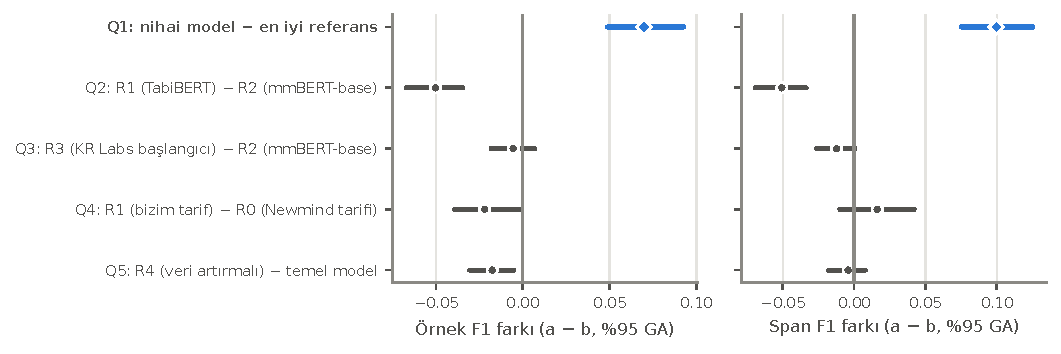
\includegraphics[width=\textwidth]{fig2_q1_q5_forest.pdf}
\caption{Önceden kaydedilmiş karşılaştırmalarda farklar (a $-$ b) ve \%95 güven aralıkları. Yalnızca Q1 doğrulayıcıdır (mavi).}
\label{fig:forest}
\end{figure*}



\subsection{Mevcut tüm dedektörlerle karşılaştırma (keşifsel)}
Nihai testte en güçlü mevcut dedektörler ModernBERT-tr ve bge-m3 olmuştur; geliştirme kümesinde seçilen TurkEmbed4STS testte geriler. Bu nedenle R2'yi mevcut yedi dedektörün her biriyle aynı yöntemle karşılaştırdık. Fark, 14 karşılaştırmanın (7 dedektör $\times$ 2 metrik) tamamında pozitif ve güven aralığı sıfırın üstündedir. En yakın rakiplere göre fark ModernBERT-tr için örnek F1'de $+0{,}028$ [0{,}008; 0{,}049] ve span F1'de $+0{,}068$ [0{,}043; 0{,}093], bge-m3 için $+0{,}037$ [0{,}018; 0{,}057] ve $+0{,}069$ [0{,}043; 0{,}096]'dır. Bu karşılaştırmalar önceden planlanmadığı ve çoklu karşılaştırma düzeltmesi içermediği için keşifsel kabul edilmelidir; doğrulayıcı iddia Q1'dir.

\subsection{Görev bazında sonuçlar}
Tablo~\ref{tab:tasks} ve Şekil~\ref{fig:tasks}, görev bazında span F1'i gösterir. R2 soru-cevap ve veriden metin görevlerinde açık farkla öndedir. Özetleme ise tüm sistemler için en zor görevdir (en iyi span F1 yaklaşık 0{,}31). Bu görevde en iyi sonucu, özetleme örnekleri içeren veri artırmalı R4 verir.

\begin{table}[t]
\centering
\caption{Görev bazında span F1 (nihai test)}
\label{tab:tasks}
\footnotesize
\begin{tabular}{@{}lccc@{}}
\toprule
Sistem & Soru-cevap & Veriden metin & Özetleme \\
\midrule
R2 (nihai) & \textbf{0,600} & 0,574 & 0,295 \\
R4 (veri artırma) & 0,587 & \textbf{0,575} & \textbf{0,309} \\
R3 & 0,599 & 0,551 & 0,283 \\
R1 TabiBERT & 0,561 & 0,497 & 0,286 \\
R0 & 0,518 & 0,529 & 0,215 \\
ModernBERT-tr & 0,544 & 0,497 & 0,238 \\
bge-m3 & 0,496 & 0,534 & 0,209 \\
TurkEmbed4STS & 0,472 & 0,503 & 0,192 \\
\bottomrule
\end{tabular}
\end{table}

\begin{figure}[t]
\centering
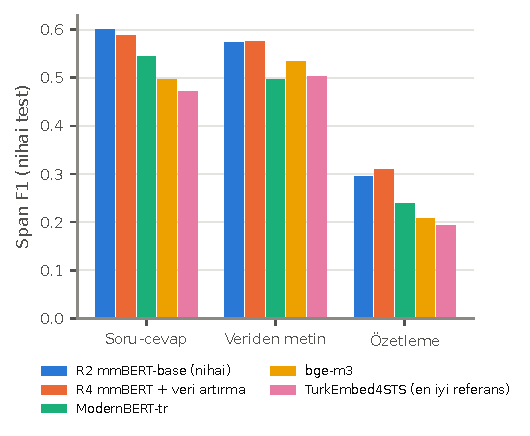
\includegraphics[width=\columnwidth]{fig3_span_f1_per_task.pdf}
\caption{Görev bazında span F1. Özetleme tüm sistemler için en zor görevdir.}
\label{fig:tasks}
\end{figure}





\begin{figure*}[t]
\centering
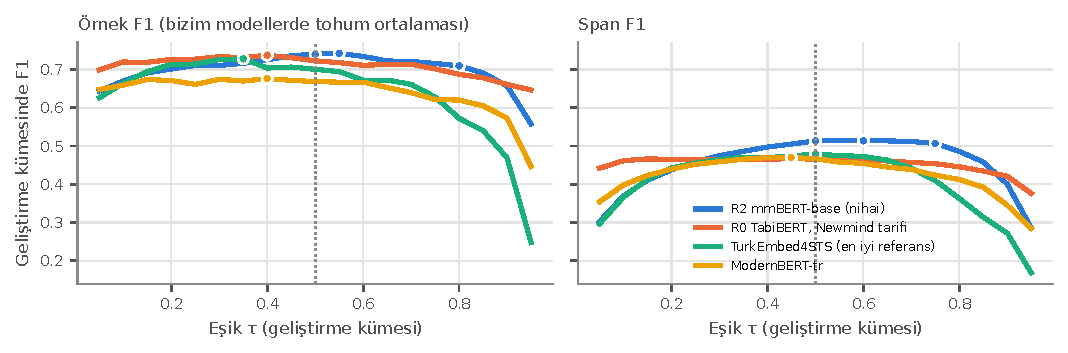
\includegraphics[width=\textwidth]{fig4_threshold_curves.pdf}
\caption{Geliştirme kümesinde eşiğe göre F1. Noktalar, her sistem için seçilip dondurulan eşiği gösterir.}
\label{fig:thr}
\end{figure*}

\begin{figure*}[t]
\centering
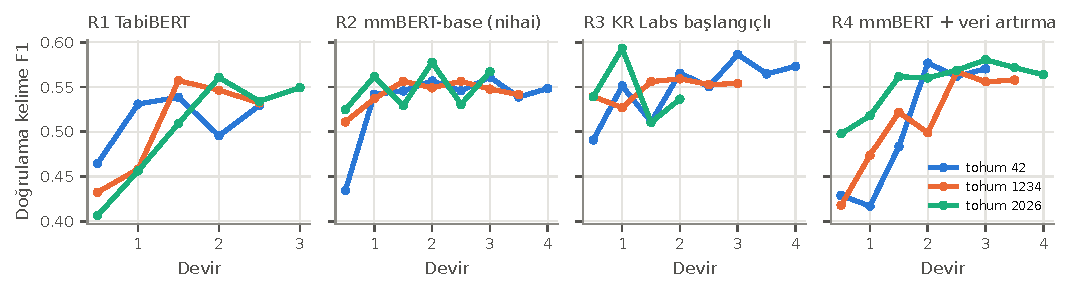
\includegraphics[width=\textwidth]{fig5_training_curves.pdf}
\caption{Her yarım devirde ölçülen doğrulama kelime F1'i (her çizgi bir tohum).}
\label{fig:train}
\end{figure*}

\subsection{Kontrollü karşılaştırmalar (Q2--Q5)}
Şekil~\ref{fig:forest} ikincil soruların etki büyüklüklerini gösterir.
\begin{itemize}
\item \textbf{Q2, temel model:} Aynı tarifle çok dilli mmBERT-base (R2), Türkçeye özgü TabiBERT'ten (R1) her iki metrikte de yaklaşık 0{,}05 puan daha iyidir (örnek F1 farkı $-0{,}050$ [$-0{,}067$; $-0{,}035$]). Yalnızca soru-cevap görevinde yapılan pilot çalışmada tersi gözlenmişti; tam veride ve üç görevde sonuç değişti.
\item \textbf{Q3, halüsinasyon ön eğitimi:} İngilizce ve diğer dillerde halüsinasyon tespiti için önceden eğitilmiş KR Labs modelinden başlamak (R3), sade mmBERT-base'den (R2) daha iyi sonuç vermedi; güven aralıkları sıfırı içerir. R3 eğitime daha hızlı başlar ama daha iyi bir noktada bitmez.
\item \textbf{Q4, eğitim tarifi:} Bizim tarifimiz (R1) ile Newmind tarzı tarif (R0) karışık sonuç verir: R0 örnek F1'de küçük bir farkla öndedir ($-0{,}022$), span F1'de fark ayırt edilemez. R1 ise kelimeleri daha iyi sıralar (kelime AUROC 0{,}897 ve 0{,}865) ve özetleme span'lerinde açıkça daha iyidir (0{,}286 ve 0{,}215). Sade kayıpla 6 devir eğitilen R0'ın olasılıkları 0 ya da 1'e yığılır; ağırlıklı kayıp ve erken durdurma daha dereceli olasılıklar üretir.
\item \textbf{Q5, veri artırma:} Çeviri testte veri artırma örnek F1'i biraz düşürür ($-0{,}018$) ve genel span F1'i değiştirmez. Özetleme span F1'i ise tüm sistemler arasında en yüksek değere çıkar. Ancak aşağıda görüleceği gibi, özgün Türkçe testte tablo tamamen değişmektedir.
\end{itemize}
Özetle, kazancın büyük kısmı temel modelden ve tüm sistemlere adil eşik verilmesinden gelir; eğitim tarifi tek başına büyük bir kaldıraç değildir.

\subsection{Eşikler ve eğitim eğrileri}
Eşik ayarı, referans dedektörlere bizim modellerimizden daha çok yardımcı olmuştur. Örneğin TurkEmbed4STS'in geliştirme kümesi örnek F1'i 0{,}5 eşiğinde 0{,}700 iken ayarlı eşikte 0{,}728'e çıkar. KR Labs sıfır atış modeli ise 0{,}5 eşiğinde neredeyse hiç işaret koymaz (test örnek F1 0{,}324), en uygun eşiği ise ızgaranın alt ucudur (0{,}05; örnek F1 0{,}551). Bu durum, modelin Türkçede kalibre olmadığını gösterir (Şekil~\ref{fig:thr}). Eğitim eğrileri (Şekil~\ref{fig:train}) doğrulama kelime F1'inin 1{,}5--2 devirde zirveye ulaştığını gösterir; erken durdurma eğitimleri genellikle 2{,}5--3 devirde sonlandırdı.

\begin{table*}[t]
\centering
\caption{Özgün Türkçe test kümesi (184 cevap, 47 halüsinasyonlu), dondurulmuş geliştirme eşikleriyle. Güven aralıkları bağlamlar yeniden örneklenerek hesaplandı. Betimseldir.}
\label{tab:native}
\footnotesize
\begin{tabular}{@{}lccccccc@{}}
\toprule
Sistem & Örnek F1 & \%95 GA & Kesinlik & Geri çağ. & AUROC & AUROC \%95 GA & Span F1 \\
\midrule
\textbf{R4 mmBERT + veri artırma} & \textbf{0,592 $\pm$ 0,018} & [0,469; 0,696] & 0,72 & 0,51 & 0,776 & [0,692; 0,851] & \textbf{0,361} \\
KR Labs v2 (sıfır atış) & 0,489 & [0,400; 0,573] & 0,33 & 0,94 & \textbf{0,826} & [0,746; 0,891] & 0,307 \\
R2 mmBERT-base (nihai) & 0,458 $\pm$ 0,079 & [0,321; 0,586] & 0,80 & 0,33 & 0,728 & [0,643; 0,809] & 0,335 \\
R3 KR Labs başlangıçlı & 0,432 $\pm$ 0,039 & [0,286; 0,560] & 0,80 & 0,30 & 0,746 & [0,661; 0,824] & 0,325 \\
R1 TabiBERT & 0,401 $\pm$ 0,047 & [0,254; 0,534] & 0,80 & 0,27 & 0,698 & [0,603; 0,784] & 0,299 \\
EuroBERT-tr & 0,400 & [0,222; 0,545] & 0,92 & 0,26 & 0,707 & [0,617; 0,791] & 0,298 \\
R0 TabiBERT, Newmind tarifi & 0,375 & [0,215; 0,525] & 0,71 & 0,26 & 0,670 & [0,576; 0,756] & 0,182 \\
bge-m3 & 0,361 & [0,200; 0,508] & 0,79 & 0,23 & 0,705 & [0,612; 0,794] & 0,228 \\
Ettin-32M & 0,337 & [0,205; 0,465] & 0,39 & 0,30 & 0,545 & [0,450; 0,643] & 0,216 \\
ModernBERT-tr & 0,310 & [0,148; 0,459] & 0,82 & 0,19 & 0,723 & [0,627; 0,808] & 0,133 \\
Kelime lojistik regresyon & 0,308 & [0,160; 0,444] & 0,56 & 0,21 & 0,699 & [0,613; 0,780] & 0,043 \\
Ettin-150M & 0,254 & [0,111; 0,393] & 0,50 & 0,17 & 0,552 & [0,448; 0,656] & 0,269 \\
TurkEmbed4STS & 0,214 & [0,077; 0,358] & 0,67 & 0,13 & 0,589 & [0,484; 0,683] & 0,079 \\
Sözcük örtüşmesi & 0,091 & [0,000; 0,197] & 0,16 & 0,06 & 0,547 & [0,454; 0,637] & 0,000 \\
\bottomrule
\end{tabular}
\end{table*}

\begin{figure*}[t]
\centering
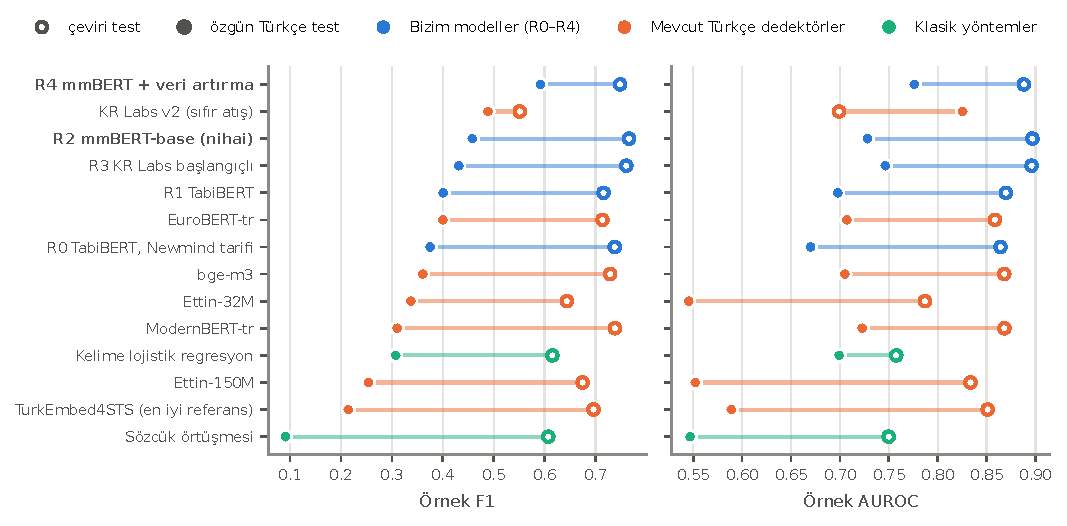
\includegraphics[width=\textwidth]{fig6_translated_vs_native.pdf}
\caption{Aynı sistemin çeviri nihai testteki (içi boş) ve özgün Türkçe testteki (dolu) başarımı. Tüm denetimli dedektörler özgün metinde belirgin biçimde düşer; en küçük düşüş veri artırmalı R4'tedir.}
\label{fig:native}
\end{figure*}

\subsection{Özgün Türkçe test kümesi (Q6)}
Özgün küme, her sistemin dondurulmuş geliştirme eşikleriyle ve yalnızca bir kez puanlandı (Tablo~\ref{tab:native}, Şekil~\ref{fig:native}). Bu analiz önceden betimsel olarak tanımlanmıştır.

\textbf{Tüm denetimli dedektörlerde büyük düşüş.} Nihai modelin örnek F1'i 0{,}766'dan 0{,}458'e, en iyi referansınki 0{,}696'dan 0{,}214'e düşer. Düşüşün ana nedeni geri çağırmadır: R2'nin işaretlediği cevaplar çoğunlukla gerçekten halüsinasyonludur (kesinlik 0{,}80), ancak halüsinasyonların yalnızca üçte birini bulur (geri çağırma 0{,}33). Özgün cevaplardaki halüsinasyonlar kısa ve incedir (yanlış yıl, bağlamdan çıkarılmış ama desteklenmeyen bir neden), çeviri eğitim verisindeki hatalara benzemez. Ayrıca çeviri geliştirme kümesinde seçilen eşikler bu veri için yüksek kalır.

\textbf{En iyi sonuç özgün Türkçe veriyle artırılmış model.} R4, örnek F1 0{,}592 [0{,}469; 0{,}696], AUROC 0{,}776 ve span F1 0{,}361 ile özgün kümede en iyi modeldir; R2'ye göre fark örnek F1'de $+0{,}134$ [0{,}037; 0{,}233]'tür. Çeviri testte etkisiz görünen veri artırma, doğal Türkçe metinde belirgin bir kazanç sağlar. Ancak Tablo~\ref{tab:subgroups}'te görüldüğü gibi bu kazancın tamamı Vikipedi alanındadır (0{,}605 ve 0{,}422); hukuk alanında iki model örnek F1'de eşittir (0{,}55) ve R4'ün AUROC'u hukukta R2'nin altına düşer (0{,}683 ve 0{,}808). Bu nedenle kazancın bir kısmı, artırma verisiyle aynı kaynaktan (Vikipedi) gelmekten kaynaklanıyor olabilir. R4, seçilen tohumdan da daha az etkilenir: R2'nin tohumlar arası standart sapması özgün kümede 0{,}079 iken R4'te 0{,}018'dir.

\textbf{Alt gruplar.} Tablo~\ref{tab:subgroups}, en önemli dört sistemi alana, üreten modele ve soru tipine göre ayırır. Halüsinasyonların toplandığı Qwen3-8B cevaplarında ve kısmen cevaplanabilir sorularda en yüksek örnek F1'i sıfır atış KR Labs modeli verir (0{,}678 ve 0{,}661); ancak bu, düşük eşiği nedeniyle çok sayıda cevabı işaretlemesinden gelir ve aynı model, neredeyse hiç halüsinasyon içermeyen DeepSeek cevaplarında da çok sayıda yanlış alarm üretir (kesinlik 0{,}05). Bağlamın tamamen cevapladığı orijinal sorularda halüsinasyon nadirdir (100 cevapta 9); burada R4 (0{,}351) R2'den (0{,}144) belirgin biçimde iyidir. DeepSeek cevaplarında yalnızca 3 halüsinasyon olduğundan bu alt kümedeki F1 değerleri anlamlı değildir.

\begin{table}[t]
\centering
\caption{Özgün kümede alt gruplara göre örnek F1 / örnek AUROC. $n$: cevap sayısı, $h$: halüsinasyonlu cevap sayısı. R2 ve R4 için 3 tohumun ortalaması. $\dagger$: $h<10$, betimsel bile değil.}
\label{tab:subgroups}
\scriptsize
\setlength{\tabcolsep}{3pt}
\begin{tabular}{@{}lrrcccc@{}}
\toprule
Alt grup & $n$ & $h$ & R2 & R4 & KR Labs v2 & ModernBERT-tr \\
\midrule
Vikipedi & 139 & 34 & 0,42 / 0,70 & \textbf{0,61} / 0,81 & 0,45 / \textbf{0,83} & 0,24 / 0,69 \\
Hukuk & 45 & 13 & 0,55 / 0,81 & 0,55 / 0,68 & \textbf{0,62} / \textbf{0,85} & 0,47 / 0,81 \\
\midrule
Qwen3-8B & 100 & 44 & 0,49 / 0,74 & 0,63 / 0,76 & \textbf{0,68} / \textbf{0,80} & 0,33 / 0,76 \\
DeepSeek$^\dagger$ & 84 & 3 & 0,00 / 0,45 & 0,00 / 0,59 & 0,10 / 0,73 & 0,00 / 0,65 \\
\midrule
Kısmi soru & 84 & 38 & 0,53 / 0,75 & 0,65 / 0,74 & \textbf{0,66} / \textbf{0,84} & 0,37 / 0,70 \\
Orijinal soru$^\dagger$ & 100 & 9 & 0,14 / 0,57 & \textbf{0,35} / \textbf{0,71} & 0,23 / 0,69 & 0,00 / 0,56 \\
\bottomrule
\end{tabular}
\end{table}

\textbf{Sıfır atış modelin sıralama başarısı.} KR Labs v2, çeviri testte en zayıf dedektörken özgün kümede en yüksek AUROC'a sahiptir (0{,}826). Ancak dondurulmuş eşiği (0{,}05) çok düşük olduğundan neredeyse her cevabı işaretler (geri çağırma 0{,}94, kesinlik 0{,}33). Aynı modelin çeviri veriyle ince ayarlanmış hâli (R3) AUROC'ta 0{,}746'ya geriler; bu da çeviri eğitim verisinin çeviriye özgü izler taşıyabileceğine işaret eder.

\textbf{Birincil karşılaştırmanın yönü korunur.} R2 ile TurkEmbed4STS arasındaki fark özgün kümede de pozitiftir (örnek F1 $+0{,}244$ [0{,}122; 0{,}363]). Diğer dedektörlerle farkların çoğunda güven aralıkları sıfırı içerir; 184 cevaplık bir küme dar aralıklar için yeterli değildir. DeepSeek cevaplarında yalnızca 3, orijinal sorularda yalnızca 9 halüsinasyon bulunduğundan bu alt kümelerde dedektörler değerlendirilemez.

% ------------------------------------------------------------------------------------------------
\section{Tartışma}

\textbf{Neden mmBERT?} TabiBERT, Türkçe metni daha az token ile kodlar ve Türkçe kıyaslama testlerinde güçlüdür. Yine de bu görevde iki kat büyük çok dilli mmBERT daha iyi sonuç verdi. Olası açıklamalar: (i) RAGTruth-TR çeviri olduğu için İngilizce yapıları taşır ve çok dilli bir model bu yapılara daha aşinadır; (ii) TabiBERT token'larının \%9'u iki kelimeye yayılır (ör. ``Ocak'a kadar'' içindeki ``a kadar''), bu da kelime sınırında etiket taşmasına yol açabilir; (iii) model boyutu farkı. Bu nedenleri ayırmak gelecekteki bir çalışmanın konusudur.

\textbf{Değerlendirme protokolünün önemi.} Aynı modeller için önceki raporlar ile bizim sonuçlarımız arasındaki farkların önemli bir kısmı değerlendirme biçiminden kaynaklanır. Eşik ayarı bazı dedektörlerde örnek F1'i 0{,}2 puandan fazla değiştirir; düzeyler (token, kelime, span, örnek) karıştırıldığında sayılar karşılaştırılamaz. Geliştirme kümesinde ``en iyi'' seçilen referansın testte gerilemesi, tek bir geliştirme puanına dayalı seçimin şans payı taşıdığını gösterir. Bu nedenle tüm kararları önceden kaydetmek ve testi bir kez açmak kritik önemdedir.

\textbf{Çeviri ile gerçek kullanım arasındaki fark.} Bu çalışmanın en önemli uyarısı, çeviri test üzerinde 0{,}7--0{,}77 örnek F1 alan dedektörlerin doğal Türkçe cevaplarda 0{,}2--0{,}6 aralığına düşmesidir. Sıralama başarısı (AUROC) daha az düşer; dolayısıyla sorunun bir kısmı kalibrasyondur ve hedef veriye yakın küçük bir kümeyle eşik ayarı yapmak pratik bir iyileştirme olabilir. Özgün Türkçe veriyle eğitim (R4) bu farkı en çok kapatan yöntemdir.

\textbf{Özgün halüsinasyonlar neye benziyor?} Tablo~\ref{tab:examples}, özgün kümeden beş tipik örnek gösterir. Özgün cevaplardaki hatalar kısadır (52 span'in ortanca uzunluğu 3 kelime, 25 karakter) ve doğal biçimde cümleye yerleşir. Örneklerde dört örüntü görülür: (i) \emph{gerçek ama desteksiz bilgi}: model dünya bilgisinden doğru bir ayrıntı ekler (ISTAT, Oscar töreninin yılı); bağlama göre bu yine de halüsinasyondur ve dedektörün ``doğru mu?'' yerine ``bağlamda var mı?'' sorusunu sorması gerekir; (ii) \emph{yakındaki bir sayıdan çıkarım}: bağlamdaki bir yıl aralığının ucu, sorulan olayın yılı olarak verilir; (iii) \emph{ilişkinin yanlış okunması}: hukuk metnindeki ``yerine'' ifadesi ``veya'' olarak aktarılır ve cezanın anlamı değişir; (iv) \emph{eksik bilgiyi tamamlama}: kısmen cevaplanabilir soruda bağlamda olmayan yıl uydurulur. Özellikle (ii) ve (iii) türlerinde cevaptaki kelimelerin hepsi bağlamda geçer; hata yalnızca kelimeler arasındaki ilişkidedir.

\begin{table*}[t]
\centering
\caption{Özgün Türkçe test kümesinden halüsinasyon örnekleri (soru ve cevaplar kısaltılmıştır; altı çizili kısım altın span'dir).}
\label{tab:examples}
\footnotesize
\setlength{\tabcolsep}{4pt}
\renewcommand{\arraystretch}{1.15}
\begin{tabular}{@{}>{\raggedright\arraybackslash}p{2.2cm}>{\raggedright\arraybackslash}p{3.9cm}>{\raggedright\arraybackslash}p{5.7cm}>{\raggedright\arraybackslash}p{5.0cm}@{}}
\toprule
Tür & Soru & Cevap (alıntı) & Bağlam ne diyor? \\
\midrule
(i) Gerçek ama desteksiz & Caserta'nın 2010 nüfusu kaçtır ve sayımı hangi kurum yapmıştır? & \ldots nüfusu 78.703'tür ve bu nüfus sayımı \uline{İtalya İstatistik Kurumu (ISTAT) tarafından yapılmıştır}. & Nüfus verilir, sayımı yapan kurum geçmez. \\
(i) Gerçek ama desteksiz & J.\ K.\ Simmons Oscar'ı hangi filmle ve hangi yıl kazandı? & \ldots 2014 yapımı \emph{Whiplash} filmindeki rolüyle \ldots\ bu ödülü \uline{2015 yılında} aldı. & Film ve yapım yılı geçer, tören yılı geçmez. \\
(ii) Yakın sayıdan çıkarım & Ankyralı Marcellus hangi yıl Roma'ya gitti? & Ankyralı Marcellus, \uline{336 yılında} Roma'ya giderek \ldots & ``314--336 yılları arasında'' episkopos olduğu söylenir; Roma yolculuğunun yılı verilmez. \\
(iii) İlişkinin yanlış okunması & Yükümlülük ihmaliyle ölüme neden olan kişiye hangi ceza verilir? & \ldots kişiye \uline{müebbet hapis cezası veya} yirmi yıldan yirmibeş yıla kadar hapis cezası verilebilir. & ``ağırlaştırılmış müebbet hapis cezası \emph{yerine} yirmi yıldan yirmibeş yıla kadar'' der. \\
(iv) Eksik bilgiyi tamamlama & Yüzde usulündeki dağıtım oranları hangi yıl yürürlüğe girmiştir? & \ldots Bakanlığınca hazırlanacak bir yönetmelikle gösterilir. Bu yönetmelik, \uline{2008 yılında yürürlüğe girmiştir}. & Oranların bir yönetmelikle gösterileceği söylenir; yıl geçmez. \\
\bottomrule
\end{tabular}
\end{table*}

\textbf{Hesaplama maliyeti.} Kodlayıcı dedektörlerin pratik avantajı hızdır: mmBERT-base tabanlı bir model, Colab GPU'sunda özgün kümenin 184 cevabını yaklaşık 6{,}6 saniyede (cevap başına $\sim$36 ms) puanlar; en küçük referans modeller cevap başına 15--20 ms'dir. Bir eğitim tek GPU'da yaklaşık bir saat sürer, veri artırmanın toplam API maliyeti 0{,}80 dolardır. Aynı işi bir BDM'ye yaptırmak her cevap için ayrı bir üretim çağrısı gerektirir.

\textbf{Sınırlılıklar.}
\begin{itemize}
\item Eğitim ve ana test verisi makine çevirisidir. Çeviri, cevapların \%3{,}5'ine etiketlenmemiş sayılar eklemiştir.
\item Özgün test kümesi küçüktür (184 cevap, 47 halüsinasyon). Etiketleri LLM ile üretilmiş, insan tarafından 50 satırlık bir örneklemde doğrulanmıştır. İnsan etiketleyici daha önce LLM etiketlerini görmüş olduğundan bu kontrol tam kör değildir ve $\kappa$ değeri ($0{,}38$) sınırlıdır. Span'ler satır satır insan tarafından düzenlenmemiştir.
\item Özgün kümede halüsinasyonların neredeyse tamamı Qwen3-8B'den ve yeniden yazılmış sorulardan gelir; bu nedenle sonuçlar bu tür halüsinasyonları temsil eder.
\item R0 tek tohumla ve farklı bir GPU'da (A100) eğitildi. Özgün küme tahminleri bf16 olarak kaydedilmiş ağırlıklarla yapıldı; iki modelde geliştirme tahminlerinden en fazla 0{,}13 olasılık farkı gözlendi.
\item Veri artırma ve özgün test aynı kaynaktan (Türkçe Vikipedi) gelir, ancak farklı makalelerdendir.
\item Veri lisansları ticari olmayan kullanımı kapsar (multi-wiki-qa: CC BY-NC-SA).
\end{itemize}

% ------------------------------------------------------------------------------------------------
\section{Sonuç ve Gelecek Çalışmalar}

Türkçe RAG cevaplarında halüsinasyon tespiti için mevcut tüm dedektörleri tek ve tekrar üretilebilir bir protokolle karşılaştırdık. Önceden kaydedilmiş birincil testte nihai modelimiz (mmBERT-base, R2) en iyi referansı her iki metrikte de anlamlı biçimde geçti ve mevcut yedi dedektörün hepsinden iyi sonuç verdi. Kontrollü deneyler, kazancın çoğunun temel modelden geldiğini gösterdi. Yeni oluşturduğumuz özgün Türkçe test kümesi ise çeviri testlerin gerçek başarımı olduğundan yüksek gösterdiğini ve özgün Türkçe veriyle eğitimin bu farkı azalttığını ortaya koydu.

Gelecek çalışmalar için: (i) özgün Türkçe eğitim verisini farklı alanlara (hukuk, sağlık) genişletmek; (ii) hedef alana yakın küçük bir kümeyle eşik ve kalibrasyon ayarı; (iii) özgün test kümesini birden fazla insan etiketleyiciyle büyütmek; (iv) üretken span dedektörleriyle~\cite{dong2026sopo,su2025rl4hs} karşılaştırma; (v) modelin ve veri kümesinin Hugging Face üzerinden yayımlanması. Tüm kod, bölmeler, etiketler ve sonuç dosyaları proje deposunda bulunmaktadır.

% ------------------------------------------------------------------------------------------------
\begin{thebibliography}{99}
\bibitem{kovacs2025lettucedetect} Á. Kovács and G. Recski, ``LettuceDetect: A hallucination detection framework for RAG applications,'' arXiv:2502.17125, 2025.
\bibitem{tas2025turk} S. Taş, M. El Huseyni, Ö. Ezerceli, R. Bayraktar, and F. B. Terzioğlu, ``Turk-LettuceDetect: A hallucination detection models for Turkish RAG applications,'' arXiv:2509.17671, 2025.
\bibitem{niu2024ragtruth} C. Niu, Y. Wu, J. Zhu, S. Xu, K. Shum, R. Zhong, J. Song, and T. Zhang, ``RAGTruth: A hallucination corpus for developing trustworthy retrieval-augmented language models,'' in \emph{Proc. 62nd Annu. Meeting Assoc. Comput. Linguistics (Vol. 1: Long Papers)}, Bangkok, Thailand, 2024, pp. 10862--10878.
\bibitem{warner2024modernbert} B. Warner \emph{et al.}, ``Smarter, better, faster, longer: A modern bidirectional encoder for fast, memory efficient, and long context finetuning and inference,'' arXiv:2412.13663, 2024.
\bibitem{belyi2025luna} M. Belyi, R. Friel, S. Shao, and A. Sanyal, ``Luna: A lightweight evaluation model to catch language model hallucinations with high accuracy and low cost,'' in \emph{Proc. 31st Int. Conf. Comput. Linguistics: Industry Track}, Abu Dhabi, UAE, 2025, pp. 398--409.
\bibitem{song2024raghat} J. Song, X. Wang, J. Zhu, Y. Wu, X. Cheng, R. Zhong, and C. Niu, ``RAG-HAT: A hallucination-aware tuning pipeline for LLM in retrieval-augmented generation,'' in \emph{Proc. EMNLP 2024: Industry Track}, Miami, FL, USA, 2024, pp. 1548--1558.
\bibitem{su2025rl4hs} H. Su \emph{et al.}, ``Learning to reason for hallucination span detection,'' arXiv:2510.02173, 2025.
\bibitem{dong2026sopo} J. Dong, Z. Bai, P. Zhu, and P. Zhou, ``SOPO: Socratic guided policy optimization for span-level hallucination detection,'' arXiv:2610.32212, 2026.
\bibitem{kovacs2026beyond} Á. Kovács \emph{et al.}, ``Beyond document grounding: Span-level hallucination detection over code, tool output, and documents,'' arXiv:2607.00895, 2026.
\bibitem{ogasa2025multiview} Y. Ogasa and Y. Arase, ``Hallucinated span detection with multi-view attention features,'' arXiv:2504.04335, 2025.
\bibitem{itkin2026temporal} I. Itkin, ``Temporal multi-signal fusion for token-level hallucination detection,'' arXiv:2608.18115, 2026.
\bibitem{kose2026ragturk} S. K. Köse \emph{et al.}, ``RAGTurk: Best practices for retrieval augmented generation in Turkish,'' in \emph{Proc. SIGTURK Workshop at EACL 2026}, arXiv:2602.03652.
\bibitem{abdaljalil2026halluversem3} S. Abdaljalil, P. Sharma, E. Serpedin, and H. Kurban, ``Halluverse-M3: A multitask multilingual benchmark for hallucination in LLMs,'' arXiv:2602.06920, 2026.
\bibitem{abdaljalil2025halluverse25} S. Abdaljalil, H. Kurban, and E. Serpedin, ``HalluVerse25: Fine-grained multilingual benchmark dataset for LLM hallucinations,'' arXiv:2503.07833, 2025.
\bibitem{turker2025tabibert} M. Türker, A. E. Kızıloğlu, O. Güngör, and S. Üsküdarlı, ``TabiBERT: A large-scale ModernBERT foundation model and a unified benchmark for Turkish,'' arXiv:2512.23065, 2025.
\bibitem{marone2025mmbert} M. Marone, O. Weller, W. Fleshman, E. Yang, D. Lawrie, and B. Van Durme, ``mmBERT: A modern multilingual encoder with annealed language learning,'' arXiv:2509.06888, 2025.
\bibitem{boizard2025eurobert} N. Boizard \emph{et al.}, ``EuroBERT: Scaling multilingual encoders for European languages,'' arXiv:2503.05500, 2025.
\bibitem{weller2025ettin} O. Weller, K. Ricci, M. Marone, A. Chaffin, D. Lawrie, and B. Van Durme, ``Seq vs seq: An open suite of paired encoders and decoders,'' arXiv:2507.11412, 2025.
\bibitem{thoresen2026multiwiki} F. Thoresen and D. S. Smart, ``A multilingual hallucination benchmark: MultiWikiQHalluA,'' arXiv:2605.02504, 2026.
\bibitem{yang2025qwen3} A. Yang \emph{et al.}, ``Qwen3 technical report,'' arXiv:2505.09388, 2025.
\end{thebibliography}

\end{document}
